% !TEX TS-program = pdflatex
% !TEX encoding = UTF-8 Unicode

\documentclass[journal,twoside,web]{IEEEmiot}
\usepackage{cite}
\usepackage{amsmath,amssymb,amsfonts}
\usepackage{algorithm}
\usepackage{algorithmic}
\usepackage{graphicx}
\usepackage[mathlines,switch]{lineno}
\usepackage{multicol,multirow}
\usepackage{marginnote}
\usepackage{stfloats}

\usepackage{mcomstd}

\usepackage{hyperref}
\hypersetup{colorlinks,
      linkcolor=nblue,
      citecolor=nblue,
      urlcolor=nblue,
      filecolor=nblue}

\usepackage{etoolbox}

\markboth{\bf More Than a Clock}{}

\title{More Than a Clock: A Connected Time and Information Display for Shared Spaces}

\author{Md~Siratul~Islam and Md~Rasedujjaman
%\thanks{}
}

\pubid{\begin{tabular}{@{}p{30pc}@{}}\\[-2pt]\multicolumn{1}{c}{2576-3180~\textcopyright~XXXX~IEEE. Applicable Copyright}\\[7pt]\end{tabular}}


\begin{document}


\maketitle


\funding{This work has been supported by funds from SUST Research Center}


\doi{10.1109/MIOT.XXXX.XXXXXX}
\DCV{XX XXXX XXXX}
\DOP{XX XXXX XXXX}


\begin{firstfootnote}
Md~Siratul~Islam is with the Department of Physics and the Department of Electrical and Electronic Engineering, Shahjalal University of Science and Technology, Sylhet 3114, Bangladesh (e-mail: siratul.islam@linux.dev)

Md~Rasedujjaman is with the Department of Electrical and Electronic Engineering, Shahjalal University of Science and Technology, Sylhet 3114, Bangladesh (e-mail: mrased-eee@sust.edu)
\end{firstfootnote}



\bodyfont

\begin{abstract}
This document provides a guide for preparing articles for IEEE \textsc{Internet of Things Magazine}. Otherwise, use this as an instruction set. The electronic file of your article will be formatted further at IEEE. Titles should be written as shown above. Avoid writing long formulas with subscripts in the title; short formulas that identify the elements are fine (e.g., “Nd–Fe–B”). Do not write “(Invited)” in the title. Full names of authors are preferred in the author field but are not required. Put a space between authors’ initials. ORCIDs should be provided here as well. In the title, all variables should appear lightface italic; numbers and units will remain bold. Abstracts must be a single paragraph. In order for an Abstract to be effective when displayed in IEEE \textit{Xplore} as well as through indexing services such as Compendex, INSPEC, Medline, ProQuest, and Web of Science, it must be an accurate, stand-alone reflection of the contents of the article. They shall not contain displayed mathematical equations, numbered reference citations, nor footnotes. They should include three or four different keywords or phrases, as this will help readers to find it. It is important to avoid over-repetition of such phrases as this can result in a page being rejected by search engines. Ensure that your abstract reads well and is grammatically correct.
\end{abstract}



\section{Introduction}
\label{sec:introduction}

A display in a shared space can change roles several times a day. It can show the time, count down a scheduled examination, become a stopwatch, and display an important notice when an announcement is needed. In corridors, offices, classrooms, examination halls, and playgrounds, these functions give people a common point of reference. These displays, if connected to a web dashboard, allow the people responsible for the space to change its content and schedule its behavior without physically accessing the device.

Providing that flexibility, however, involves more than simply sending text to a screen. If it's a notice, it can be easily delivered as a remote command. But when it's a scheduled countdown/countup, it must progress locally once its timing information has been received. The device needs to retain enough information to restore its intended behavior after a restart. For example, restarting a display during an examination should not reset the countdown or extend the scheduled interval. Installation and maintenance introduce further requirements: users need a way to configure connectivity, and firmware updates must be possible after the display has been mounted. We address these requirements through an Internet of Things (IoT) system.

We developed a connected time and information display that includes selectable clockfaces, scrolling notices and alerts, a stopwatch, scheduled count-up and countdown features. Users manage the devices through a web dashboard, which communicates with them over Wi-Fi using the Message Queuing Telemetry Transport (MQTT) protocol. Each device executes its display and timing functions locally. The implementation combines an ESP32-S3 controller running Zephyr RTOS with chained HUB12 LED matrix display panels and a custom PCB. Network time synchronization, a real-time clock, persistent settings, Wi-Fi configuration through access point (AP) mode, and over-the-air updates using signed firmware support operation after installation.

\begin{figure}[t]
\centering
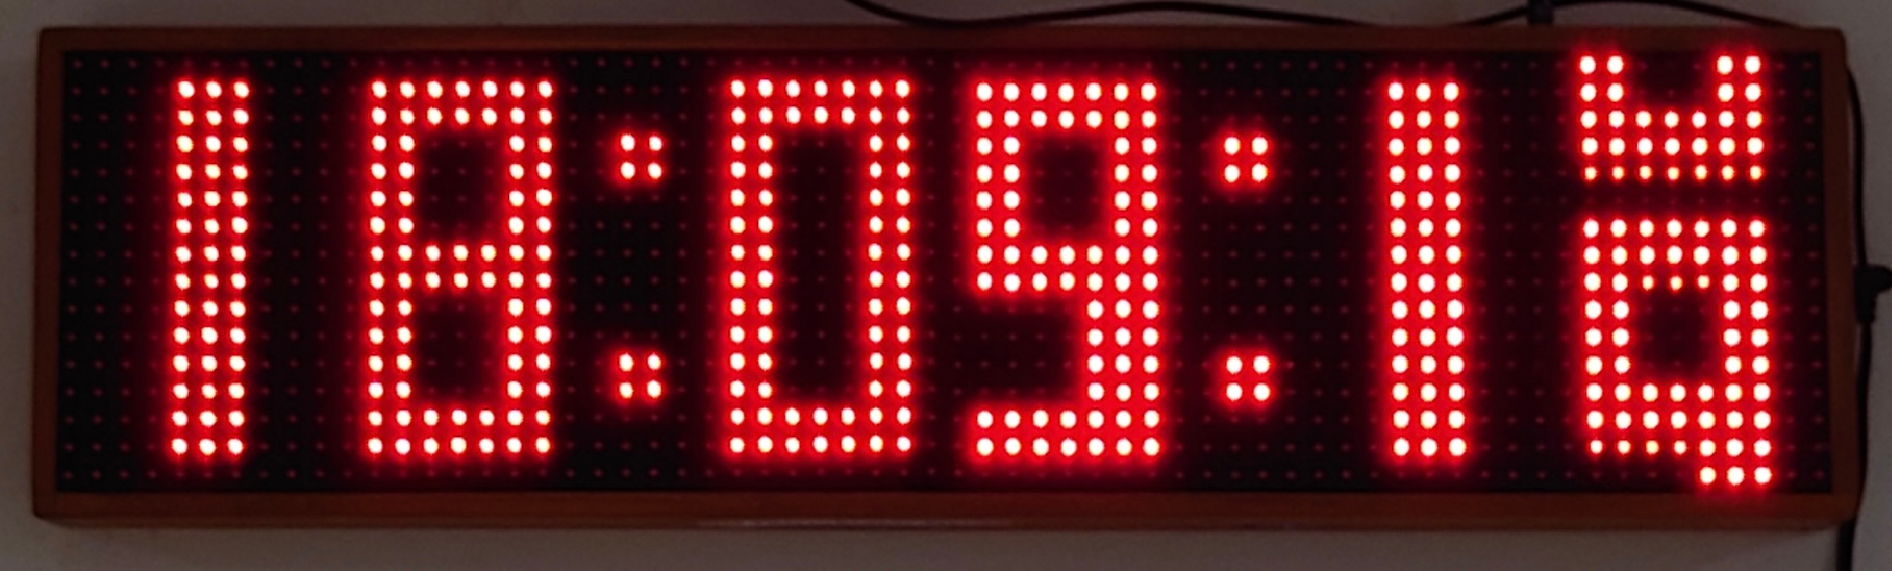
\includegraphics[width=\columnwidth]{figs/clock.pdf}
\par\vspace{1pt}
{\footnotesize (a) Clock}\par\medskip
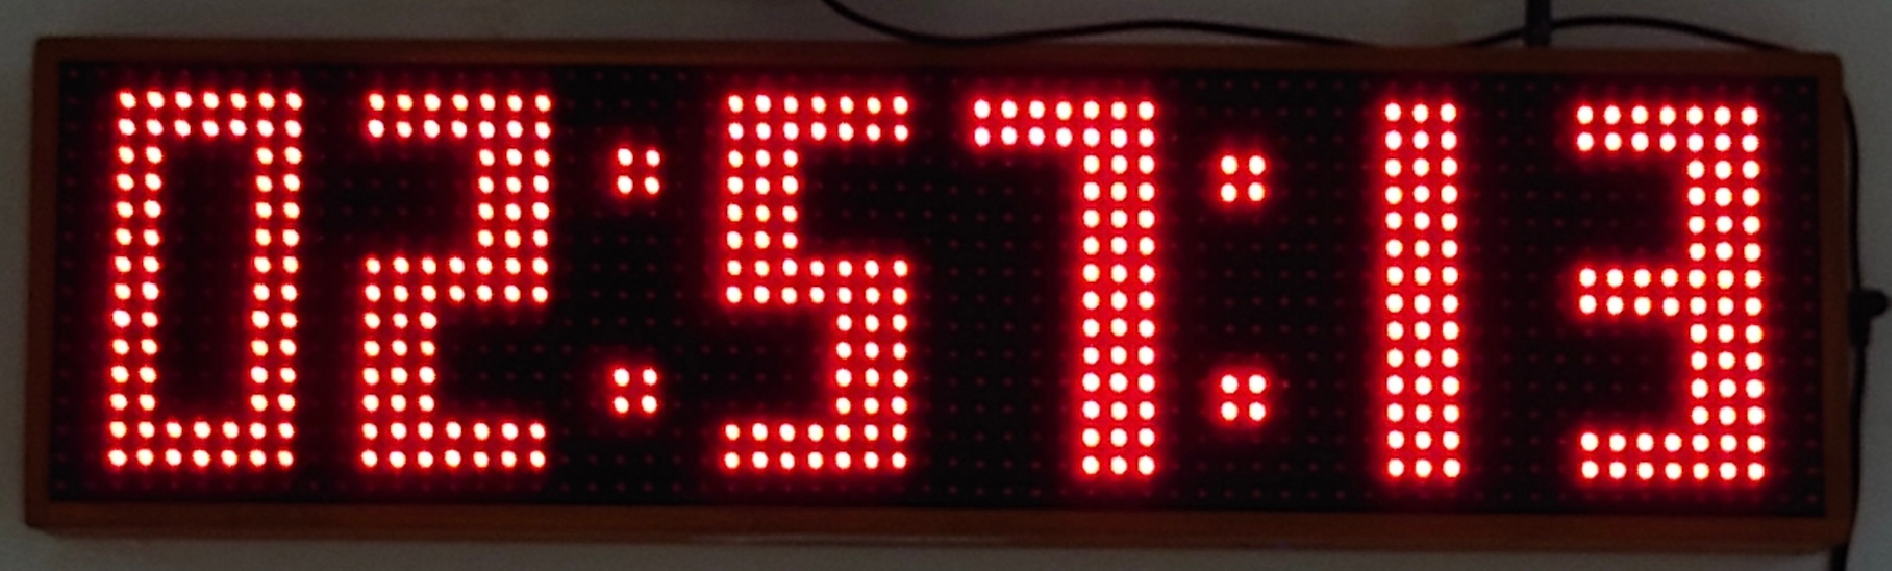
\includegraphics[width=\columnwidth]{figs/timer.pdf}
\par\vspace{1pt}
{\footnotesize (b) Countdown}\par\medskip
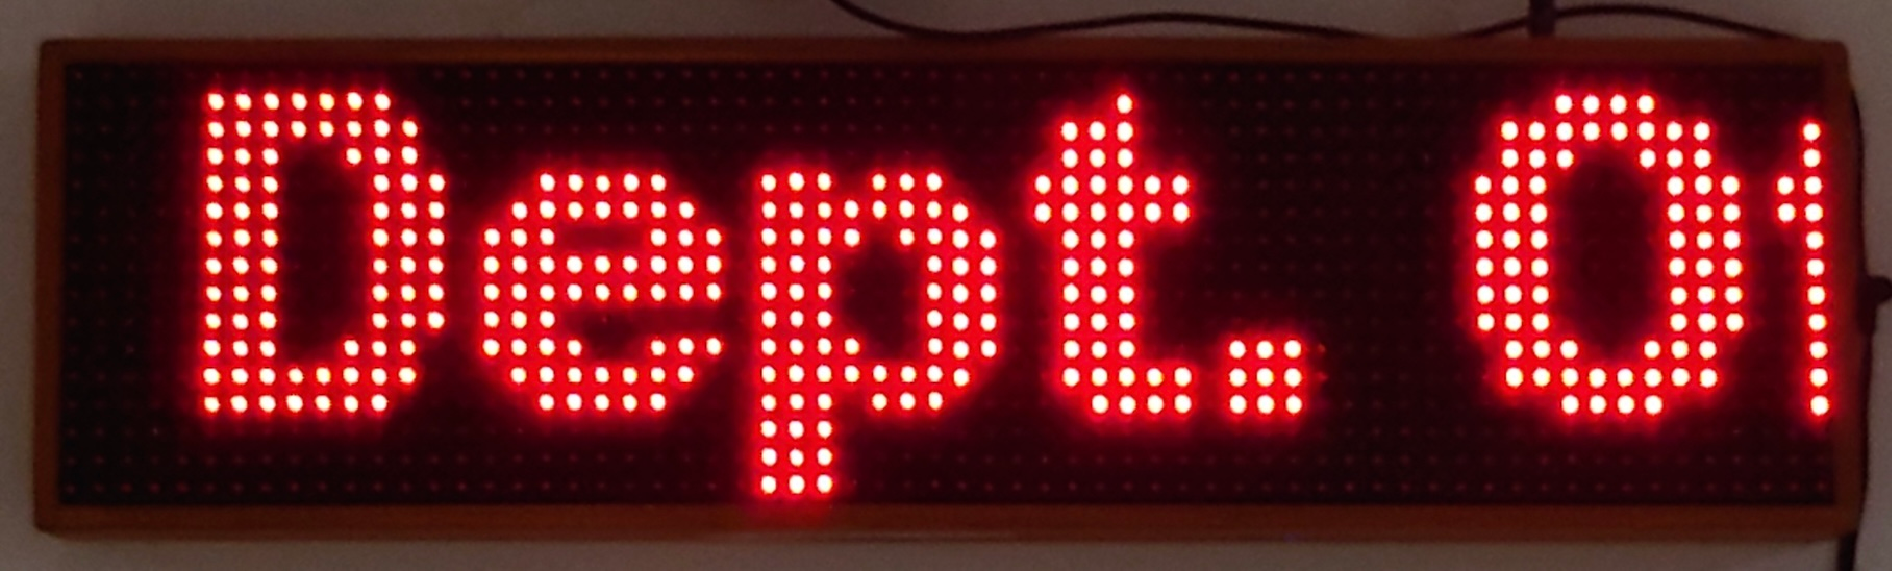
\includegraphics[width=\columnwidth]{figs/notice.pdf}
\par\vspace{1pt}
{\footnotesize (c) Scrolling notice}
\caption{An installed display operating in three modes.}
\label{fig:display}
\end{figure}

We deployed ten units at Shahjalal University of Science and Technology, Bangladesh (Fig.~\ref{fig:display}). Teachers and staff use the displays for timekeeping, announcements, important notices, and examination scheduling in spaces ranging from corridors and offices to classrooms and examination halls.
\section{Related Work}
\label{sec:related_work}

Connected displays have been developed for activity timing and information sharing in public spaces. Kumar et al.~\cite{kumar2023noticeboard} developed a web controlled noticeboard using an ESP8266-based NodeMCU and 8$\times$8 LED matrix displays. Their interface supports showing messages and controlling scrolling speed and direction. Our system uses two chained 32$\times$16 P10 display large enough for distant viewing, and supports more features including everyday timekeeping, stopwatch, and scheduled count-up and countdown functions. It also integrates device-hosted network configuration and signed firmware updates, which are not described in their implementation.

Kader et al.~\cite{kader2019timing} developed an Arduino Uno-based system for managing viva and presentation sessions. It combines a countdown and buzzer alerts with a separate display that shows group numbers and information to waiting candidates. The examiner operates the system through an IR remote, while an RF link connects the display units, with reported operating ranges of 7~m and 11~m, respectively. Our system uses chained HUB12 panels to provide a large display for timekeeping, notices, and scheduled activities, with management through a web dashboard which is accessible from anywhere with internet access.

Sethi et al.~\cite{sethi2015management} developed a cloud-connected signage management system using Linux-based displays, with phone-assisted provisioning and remote administration through SSH and VNC. Our design targets low-cost MCU  with as much control as we can feasibly get. We use an ESP32-S3 running Zephyr RTOS. This avoids requiring a Linux-capable display controller and browser-based rendering on each device.

Memarovic et al.~\cite{memarovic2016networked} reported the development and deployment of a university display network but their work emphasizes stakeholder involvement and deployment. Their study provides context for introducing displays into shared institutional spaces. Our article focuses on the embedded hardware and software that support timekeeping, announcements, scheduled activities, and maintenance, drawing on ten deployed units operated by teachers and staff.

To the best of our knowledge, prior works do not describe a microcontroller-based display that combines (i) everyday timekeeping, scrolling notices and alerts, stopwatch operation, and scheduled count-up and countdown functions; (ii) web-based content and schedule management with local timing execution and persistent configuration; (iii) device-hosted Wi-Fi provisioning with network scanning and management of up to five saved network profiles; and (iv) over-the-air updates using signed firmware. Our implementation integrates these capabilities on an ESP32-S3 running Zephyr RTOS. We additionally contributed the HUB12 display driver to upstream Zephyr, making it reusable beyond this system.

We also designed and built a custom carrier PCB connecting the controller, RTC, display interface, and power stage, along with a separate board for local controls and status indicators.
\section{Design Philosophy and System Architecture}
\label{sec:system_overview}

The design brings several everyday functions into a display that users can configure and maintain after installation. A teacher may use it for an examination countdown, while office staff may use the same device for a notice or ordinary timekeeping. Changing its role should require changing its configuration through a browser. This guided the choice to combine display functions, network setup, persistent configuration, and firmware maintenance within one microcontroller-based system.

\begin{figure*}[t]
\centering
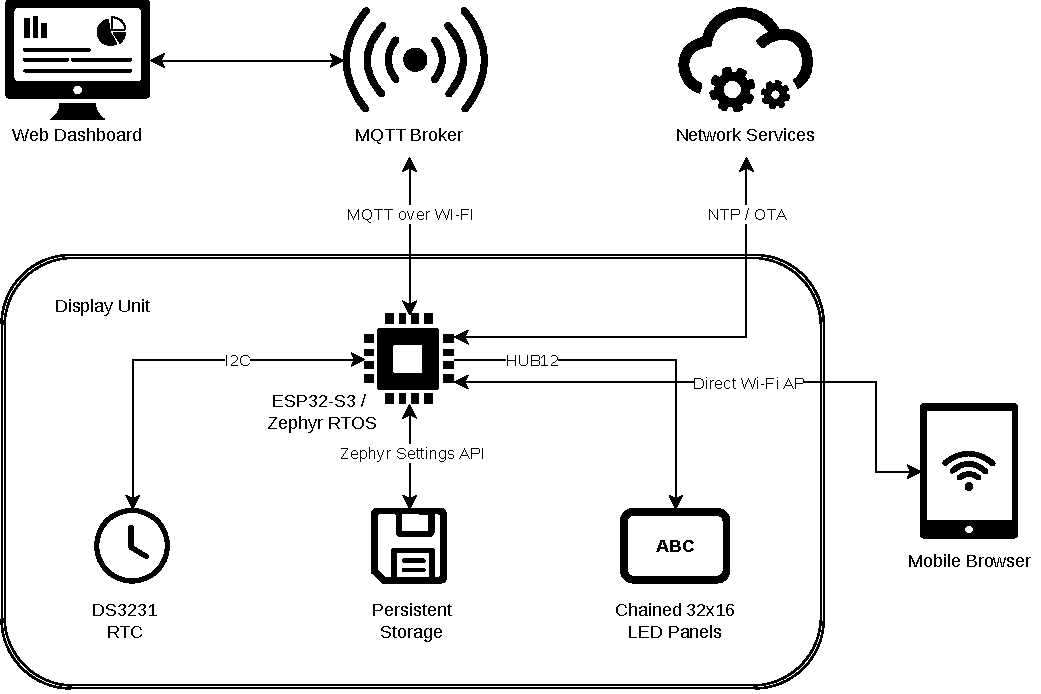
\includegraphics[width=\textwidth]{figs/architecture.pdf}
\caption{System architecture combining remote management with local display execution. The mobile browser provides a direct connection for Wi-Fi provisioning, while network services supply time synchronization and firmware images.}
\label{fig:architecture}
\end{figure*}

Figure~\ref{fig:architecture} shows how these responsibilities are distributed. The web dashboard provides the management interface, and MQTT carries commands and device status. The ESP32-S3 interprets these commands and generates the displayed content locally. Clockfaces, scrolling notices, and timers share a display manager and framebuffer, with the chained panels presented through Zephyr's display interface. The same display also presents firmware-update progress. This arrangement supports the required text and timing functions without a Linux-capable controller or browser-based rendering on each unit.

Local execution includes deciding how an activity progresses over time. A scheduled timer is represented by its start and end timestamps, which are retained in persistent storage. During startup, the firmware compares these timestamps with the RTC: a future activity remains scheduled, an active activity resumes according to the current time, and an expired activity is cleared. For example, a countdown scheduled to finish at 11:00 should still finish at 11:00 after a restart at 10:20. Preserving the schedule therefore matters more than preserving the last number drawn on the screen.

Zephyr provides a common software foundation through its device interfaces, networking facilities, and settings subsystem. The chained panels are exposed through its display interface, keeping the application independent of the panel-driving details. We contributed the HUB12 driver to upstream Zephyr, allowing the panel interface to be reused independently of the clock application.

Installation and maintenance shaped the design alongside its display functions. Users need to connect a mounted unit to the local network, change its role, and install software updates without opening the enclosure. We therefore included browser-based provisioning and remote firmware updates as part of the device's normal operation.
\section{Hardware Design}
\label{sec:hardware}

Building multiple units for installation in different rooms calls for a repeatable assembly and controls that remain accessible once the display is enclosed. The custom carrier PCB in Fig.~\ref{fig:hardware} brings the ESP32-S3 development board, RTC module, power converter, and HUB12 display connector into one assembly with fixed connections and mounting positions. A separate narrow board carries the AP-mode button and status indicators and connects to the controller through a five-pin cable. This arrangement allows the controls to be positioned independently of the main board, giving users access to network setup and device status from the outside of the enclosure.

\begin{figure*}[t]
\centering
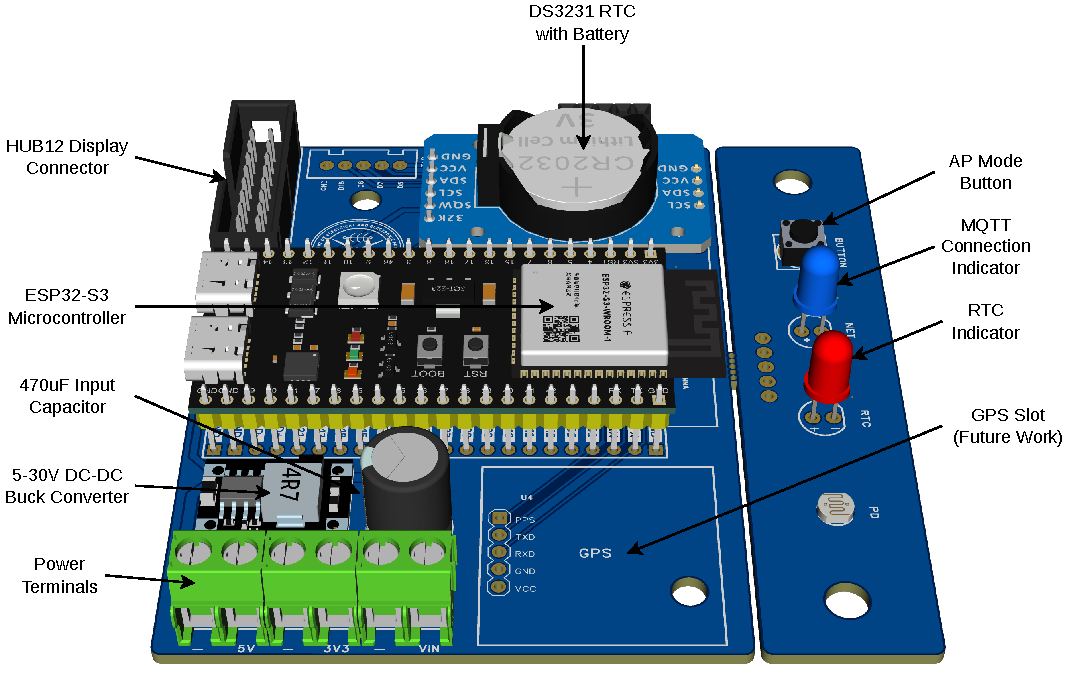
\includegraphics[width=\textwidth]{figs/hardware.pdf}
\caption{Custom controller and user-interface boards, showing the display connection, battery-backed RTC, power stage, and local controls. The GPS slot is reserved for future expansion.}
\label{fig:hardware}
\end{figure*}

The deployed units use two chained $32 \times 16$ P10 LED panels, forming a $64 \times 16$ display. Large digits occupy most of the available height during timekeeping and countdown operation, while longer notices scroll across the same surface. The limited resolution encourages a simple presentation of large characters and animations, with detailed configuration handled through the web dashboard. The HUB12 driver also supports horizontal chaining beyond two panels, allowing wider displays to be built for other installations. Adding panels increases the space available for content while retaining the same 16-pixel height.

Power arrangements can also vary between installations. The board uses a DC--DC buck converter configured for a 5~V output, allowing a higher-voltage DC adapter to supply the required rail. Where a regulated 5~V supply is already available, the converter can be omitted and the bypass connection populated. Screw terminals provide connections for VIN, 5~V, and 3.3~V, while a 470~$\mu$F capacitor across VIN and ground provides input bulk capacitance. These options allow the same PCB to accommodate different supply arrangements.

A DS3231 RTC connected over I$^2$C maintains the local time reference, with a backup battery preserving time while the main supply is disconnected. When power returns, the controller can read the current time before network synchronization becomes available. Together with schedules retained in flash, this provides the hardware basis for the restart behavior described in the \nameref{sec:system_overview} section.
\section{Software and Remote Operation}
\label{sec:software}

Once a display is mounted, changing its purpose should be an ordinary task for the people using the room. A teacher preparing an examination needs to set a countdown, office staff need to publish a notice, a maintainer needs to update the firmware. The software supports these activities through a device-hosted configuration page and a remote web dashboard, while the microcontroller handles the displayed content and timing.

\subsection{Connecting an Installed Display}

Network setup begins at the display itself. Holding the local button activates AP mode, allowing a phone to connect directly to the device. The user then opens the device's IP address in a browser, scans nearby Wi-Fi networks, and supplies the required credentials. The portal lists networks by signal strength and identifies saved entries. Up to five network profiles are retained in flash, allowing credentials to survive a restart.

The configuration page and its HTTP server are implemented within the Zephyr application. This gives the device a setup interface before it has access to the dashboard or external network services. After provisioning, the user can reconnect the phone to its normal network and open the dashboard in the same browser. No dedicated mobile application or programming cable is required.

\subsection{Changing the Display's Role}

The dashboard provides controls for clockface selection, notices, and timers. Figure~\ref{fig:dashboard} shows two common tasks. For a timer, the user chooses a duration, selects count-up or countdown operation, and requests an immediate or scheduled start. The interface also lists scheduled activities with their start and end times. For a notice, the user enters the message and selects its display duration or date-and-time interval.

\begin{figure*}[t]
\centering
\begin{minipage}[b]{0.49\textwidth}
\centering
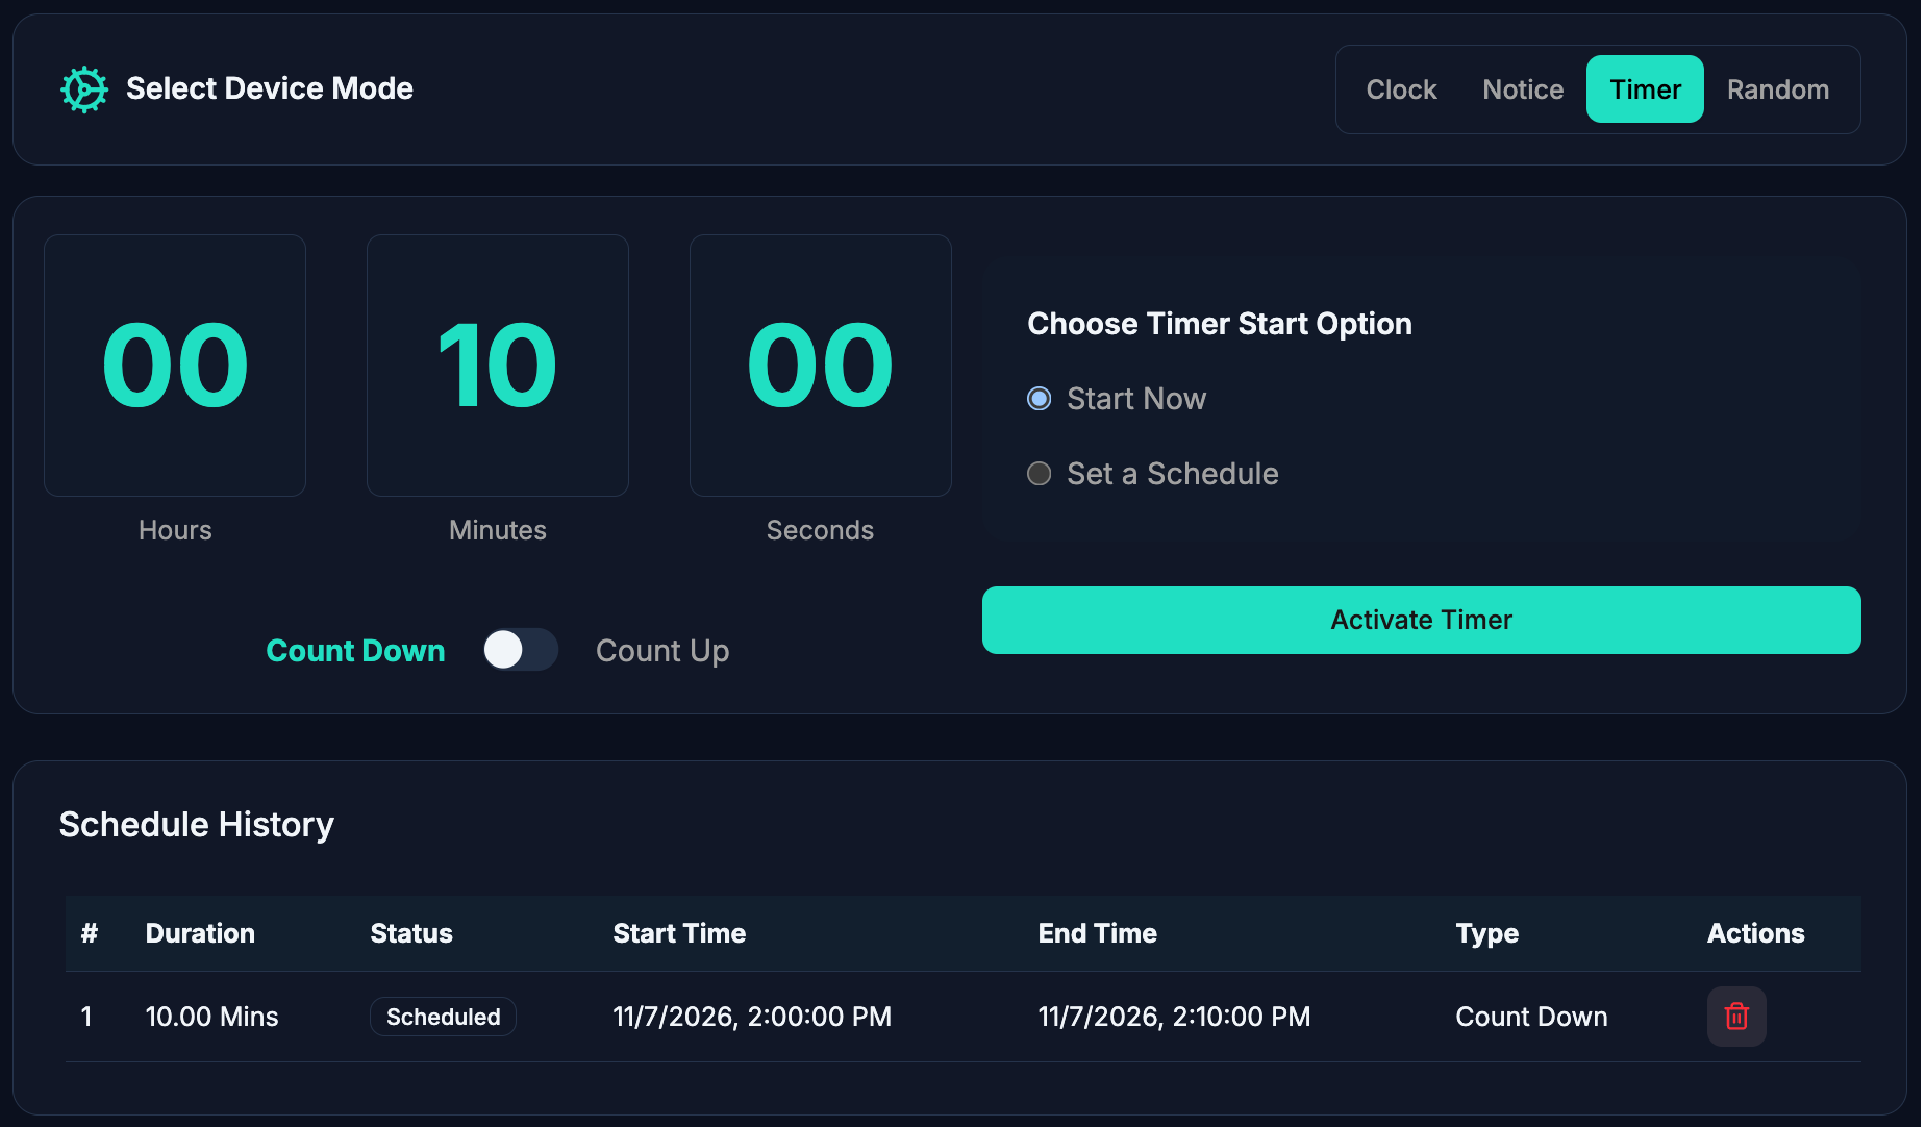
\includegraphics[width=\linewidth]{figs/dashboard_timer}
\par\vspace{2pt}
{\footnotesize (a) Timer control}
\end{minipage}
\hfill
\begin{minipage}[b]{0.49\textwidth}
\centering
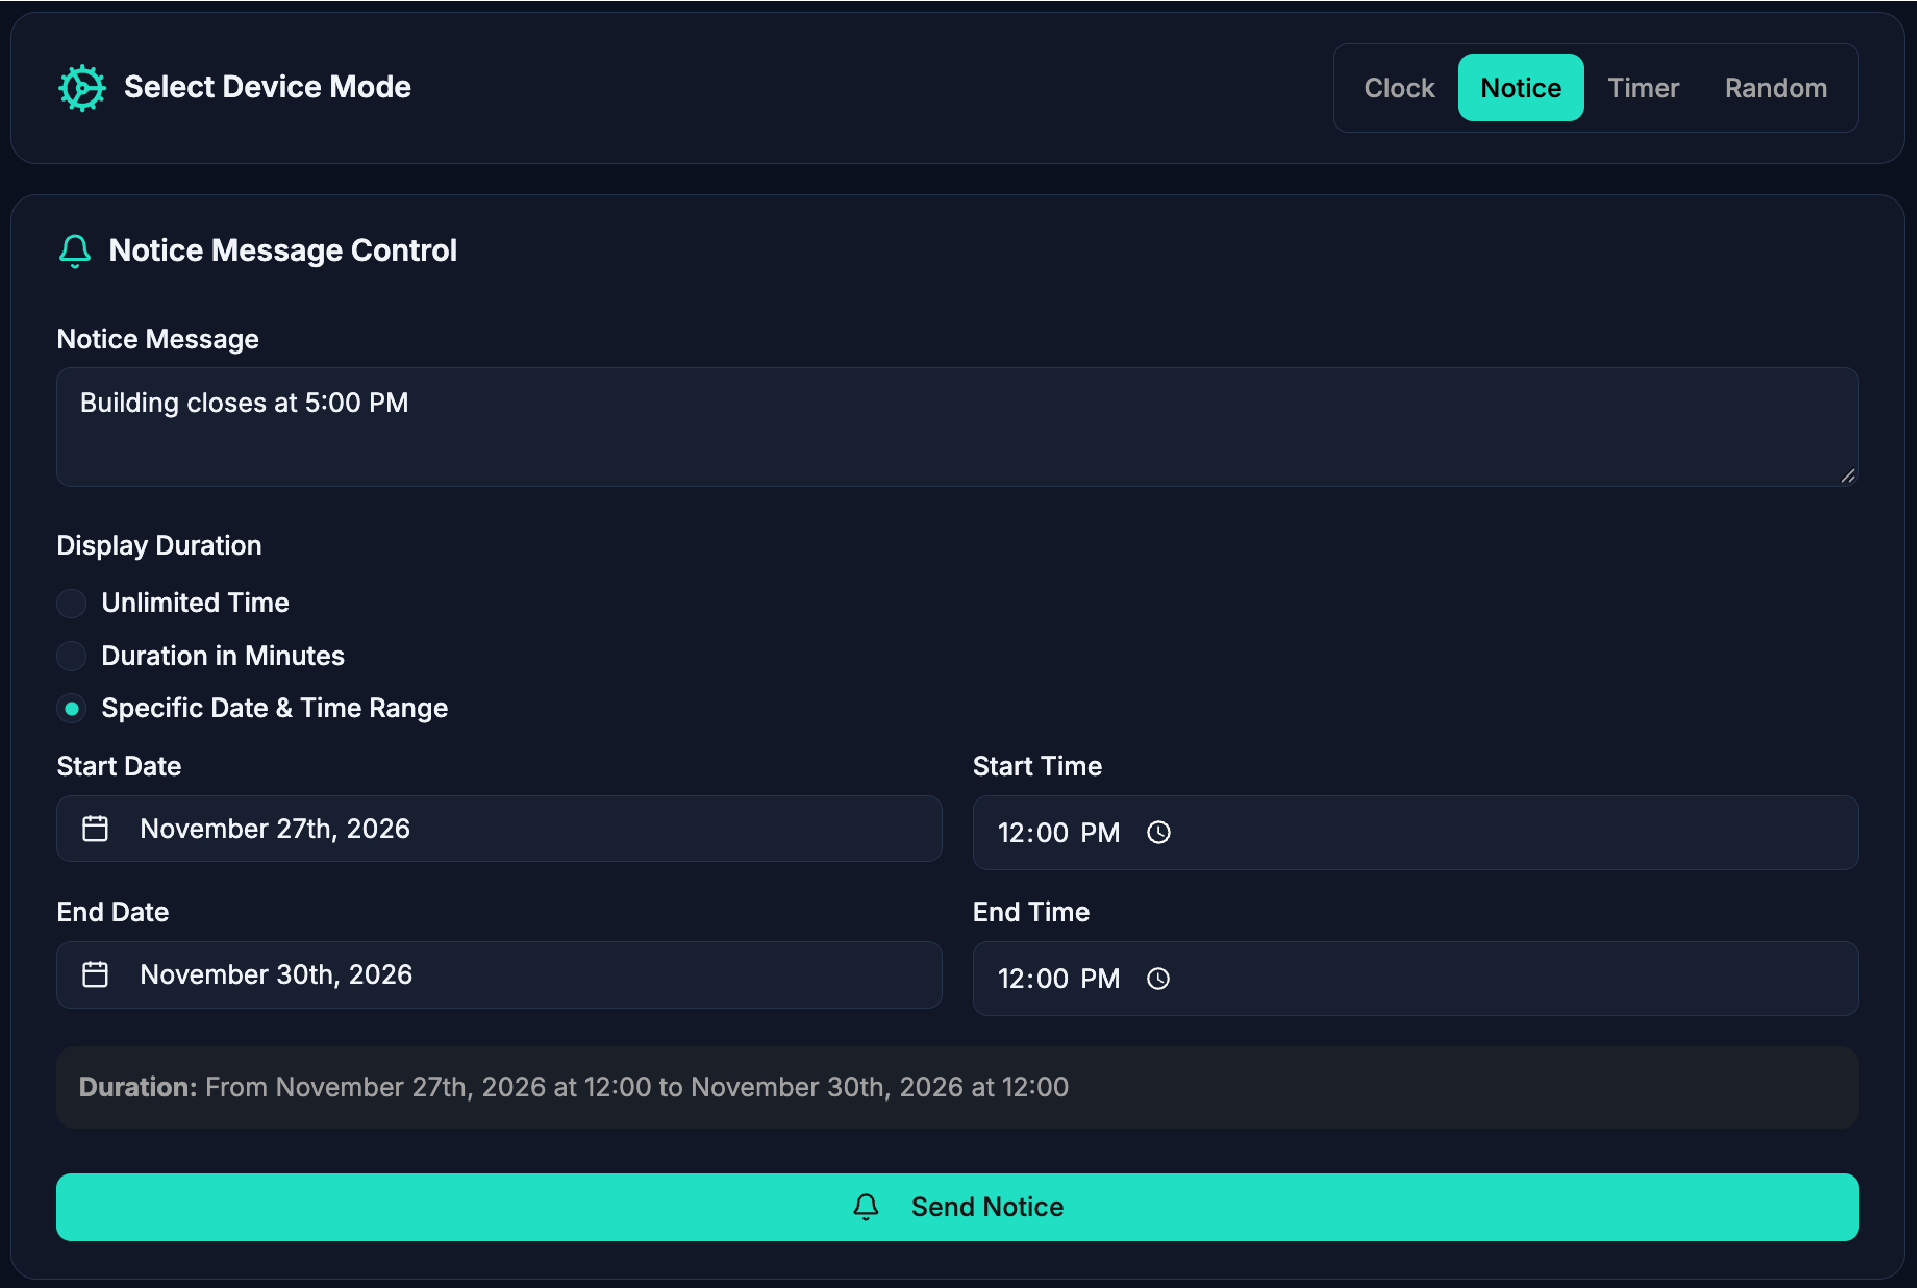
\includegraphics[width=\linewidth]{figs/dashboard_notice}
\par\vspace{2pt}
{\footnotesize (b) Notice scheduling}
\end{minipage}
\caption{Web dashboard interfaces for (a) configuring timers and viewing scheduled activities and (b) composing notices with a specified display interval.}
\label{fig:dashboard}
\end{figure*}

MQTT carries commands to the selected device, which generates the displayed content locally. Users can change clockfaces, publish notices, and configure timed activities through the dashboard. The dashboard also exposes device status, the reported operating mode, and firmware version, helping users identify the unit they are managing.

\subsection{Keeping Display Operation Responsive}

Network activity and display rendering have different rhythms. A connection attempt may take seconds, while scrolling text needs frequent updates. The application therefore handles Wi-Fi connection management and MQTT processing separately from the display thread. Network connection attempts proceed in the background, and the display thread renders the current mode into a shared framebuffer.

The application retains settings such as the selected clockface, notice text, brightness, and timer timestamps. These saved values support restoration after a restart, including the schedule recovery described in the \nameref{sec:system_overview} section. Network time synchronization updates the RTC when connectivity is available.

\subsection{Updating Firmware After Installation}

Firmware maintenance follows a similar remote workflow. An update command supplies the firmware image URL, and the device downloads the image into a secondary flash slot. During the transfer, the LED panels show update progress, giving someone near the display a visible explanation for the interruption to normal operation. Progress and error messages are also published over MQTT.

After staging the image, the application requests an MCUboot test upgrade and restarts. MCUboot validates the image signature before allowing the new firmware to run. This permits software changes after installation while checking that the replacement image was signed with the expected key.

\bibliographystyle{IEEEtran}
\bibliography{references}


\section{Biographies}
\vspace*{-30pt}

\begin{biography}[{\parbox[b][1.25in][t]{1in}{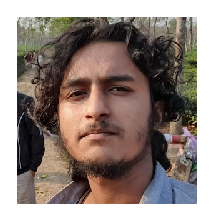
\includegraphics[width=1in,height=1.25in,keepaspectratio]{sirat}}}]{Md~Siratul~Islam} is pursuing the B.Sc. degree in Physics and serves as a Research Assistant in Electrical and Electronic Engineering at Shahjalal University of Science and Technology, Bangladesh. He authored and maintains Zephyr's FIDO2 and biometrics subsystems, maintains Linux drivers, and reviews IIO patches.
\end{biography}

\begin{biography}[{\parbox[b][1.25in][t]{1in}{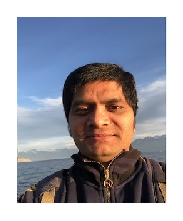
\includegraphics[width=1in,height=1.25in,keepaspectratio]{resedujjaman}}}]{Md~Rasedujjaman}
is with the Department of Electrical and Electronic Engineering, Shahjalal University of Science and Technology, Bangladesh.
\end{biography}


\vfill
\end{document}

